%===================================== CHAP 5 =================================

\chapter{Results}

This chapter presents the results of the test cases described in the previous chapter.

\section{CASE 1: Inferring constant weights with Newton method}
Figure \ref{fig:Newton} illustrates the log-likelihood function, and the points for the initial guess and the two first iterations in the Newton method.


\begin{figure}[hbt!]
\caption{}
\label{fig:Newton}
    \centering
    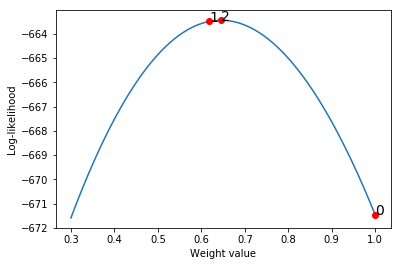
\includegraphics[scale=0.8]{Newton_method.png}
\end{figure}

The method saturates after two iterations. 

\section{Inferring dynamic weights}

\textsc{Starting iterations from true weights}\\
For the first case the true weight trajectory is plotted in the following figure. 


\begin{figure}[hbt!]
    \centering
    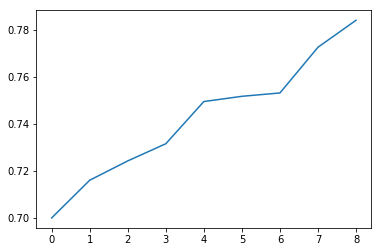
\includegraphics[scale=0.8]{Underlying.png}
\end{figure}

The following plot shows the normalized mean squared error when using different number of trials, starting the iterations from the correct weights. The variance used in the proposal and prior distribution is equal to $0.0001$. The number of iterations was 3000.

\begin{figure}[hbt!]
    \centering
    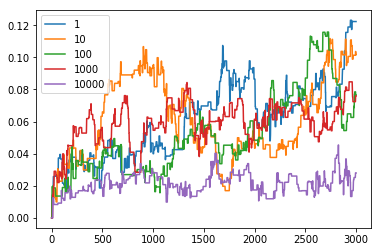
\includegraphics[scale=0.8]{MSE3.png}
\end{figure}

The same was done 100 times for each number of trials. The underlying weights were drawn new for each replicate. The following plot shows the mean of the MSE values at each iteration, with variance bars around it. 

\begin{figure}[hbt!]
    \centering
    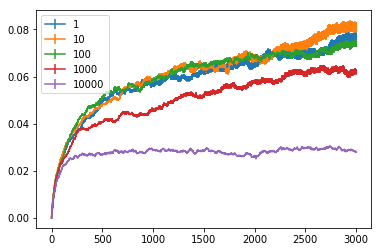
\includegraphics[scale=0.8]{Mean_plot_std.png}
\end{figure}

The standard deviation bars were 

\begin{figure}[hbt!]
    \centering
    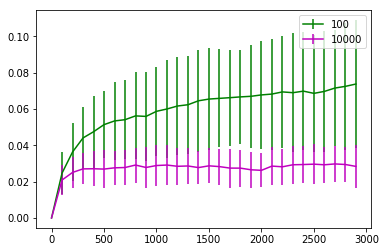
\includegraphics[scale=0.8]{Std_every100.png}
\end{figure}

\textsc{Starting weight trajectory different from true weights}
It is also interesting to see how well the algorithm manages to find the actual weights when the iterations begins from somewhere else. Now the initial guess for the MCMC iterations is set to be a random walk around 1.

\begin{figure}[hbt!]
    \centering
    \includegraphics[scale=0.8]{Start_it_1000.png}
\end{figure}


\begin{figure}[hbt!]
    \centering
    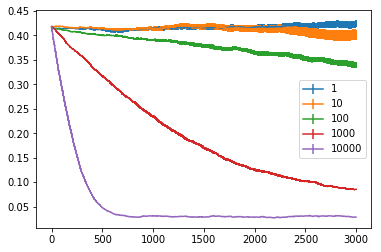
\includegraphics[scale=0.8]{MSE_starting_away.png}
\end{figure}

Figure \ref{w_trajectory_1000} and  shows how the weight trajectory develops over the iterations for 100 and 1000  (Note to myself: appendix? Since these are weight trajectories for single iterations their look is quite random. Maybe change to average weight trajectory of 100 or something?)

\begin{figure}[hbt!]
    \centering
    \includegraphics[scale=0.3]{fig/Start_it_1000.png}
    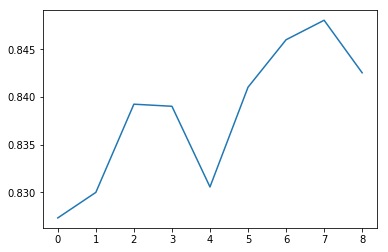
\includegraphics[scale = 0.3]{fig/1000_it_1000.png}
    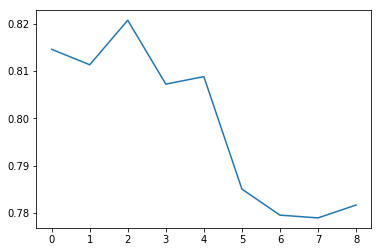
\includegraphics[scale = 0.3]{fig/2000_it_1000.png}\\
    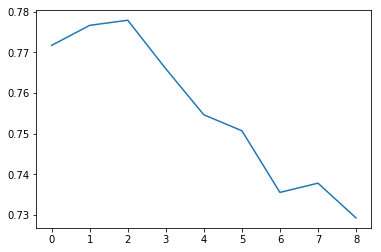
\includegraphics[scale = 0.3]{fig/3000_it_1000.png}
    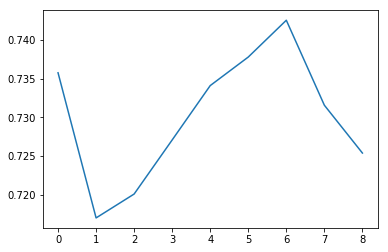
\includegraphics[scale = 0.3]{fig/4000_it_1000.png}
    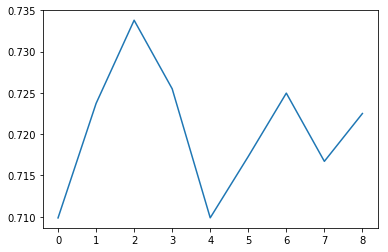
\includegraphics[scale = 0.3]{fig/5000_it_1000.png}
    \caption{Development of weight trajectory over iterations for 1000 trials. 0, 1000, 2000, 3000, 4000 and 5000 iterations}
    \label{w_trajectory_1000}
\end{figure}

\begin{figure}[hbt!]
    \centering
    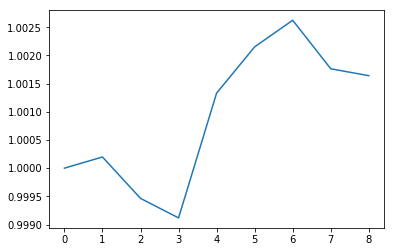
\includegraphics[scale=0.3]{fig/Start_it_100.png}
    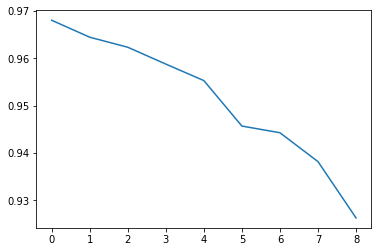
\includegraphics[scale = 0.3]{fig/1000_it_100.png}
    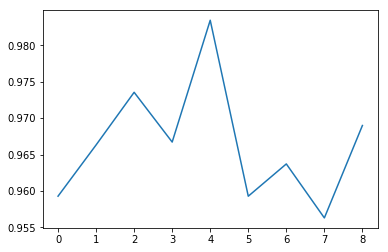
\includegraphics[scale = 0.3]{fig/2000_it_100.png}\\
    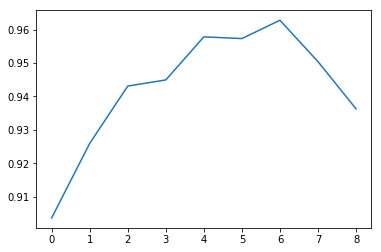
\includegraphics[scale = 0.3]{fig/3000_it_100.png}
    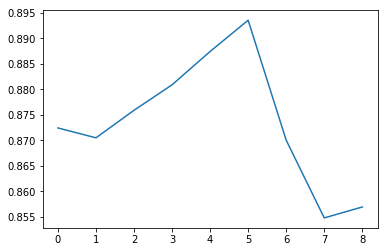
\includegraphics[scale = 0.3]{fig/4000_it_100.png}
    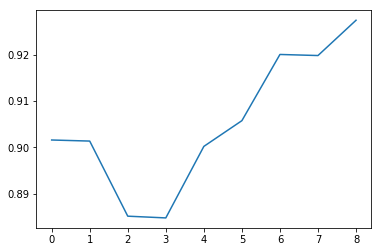
\includegraphics[scale = 0.3]{fig/5000_it_100.png}
    \caption{Development of weight trajectory over iterations for 100 trials. 0, 1000, 2000, 3000, 4000 and 5000 iterations}
    \label{w_trajectory_1000}
\end{figure}

\section{Weights generated by learning rule}

\begin{itemize}
    \item Describe test case and how I generated the weights
    \item Figures with results. Trying different variances for the prior ect
\end{itemize}

\begin{figure}[hbt!]
    \centering
    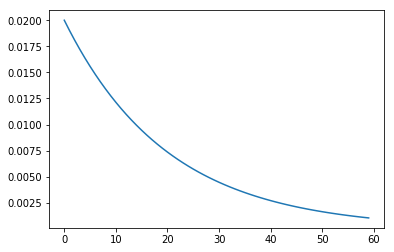
\includegraphics[scale=0.8]{Learning_rule.png}
\end{figure}

\cleardoublepage